%%
% The BIThesis Template for Bachelor Graduation Thesis
%
% 北京理工大学毕业设计(论文)第一章节 —— 使用 XeLaTeX 编译
%
% Copyright 2020 Spencer Woo
%
% This work may be distributed and/or modified under the
% conditions of the LaTeX Project Public License, either version 1.3
% of this license or (at your option) any later version.
% The latest version of this license is in
%   http://www.latex-project.org/lppl.txt
% and version 1.3 or later is part of all distributions of LaTeX
% version 2005/12/01 or later.
%
% This work has the LPPL maintenance status `maintained'.
%
% The Current Maintainer of this work is Spencer Woo.
%
% 第一章节

\chapter{史瓦西黑洞物理}
\section{黑洞简介}
\subsection{黑洞是什么}
黑洞是一片引力强大到连光都无法逃脱的区域\cite{what_is_black_hole}。银河系的中心就是一个质量为太阳430万倍的黑洞\cite{galactic_center_bh},几乎所有的星系中心都是一个超大质量的黑洞。
\subsection{奇点}
黑洞的中心是一个密度无穷大的奇点,奇点的时空也无限扭曲。黑洞奇点是造成时空扭曲并形成黑洞视界的根源。
\subsection{事件视界}
黑洞的视界是使黑洞称为黑洞的区域,视界以内的信息都无法向外传递,因为没有向外的路径存在。本文研究的限制在视界以外的区域(exterior)。
\subsection{引力透镜}
黑洞(事件视界)根据无毛定理,任何信息都不能从视界上发射出来\footnote{不考虑量子力学},导致黑洞本身是不能被看到的。但黑洞会扭曲周围的时空,通过观察周围物质的运动可以“看”到黑洞。\\
黑洞就像一个圆形或者近似圆形透镜,会使远处传来的平行光产生偏折。

\section{描述弯曲的时空}
\subsection{时间与空间}
狭义相对论开始,时间与空间在洛伦兹变换下被密切的关联起来。从光速不变原理引出长度收缩与时间膨胀的现象。闵可夫斯基时空将时间作为坐标的一个维度,构建了一个四维的坐标系$\left(ct,x,y,z\right)$。刘慈欣在三体中写道,「光锥之内就是命运」\cite{three-body},即是说你所在时空所有光锥之外的事件都与你无关。

\subsection{黎曼几何}
闵可夫斯基时空是一个平直的时空,仅适用于狭义相对论。广义相对论中,时空不再是平直的。要描述一个扭曲的时空,就要用到非欧几何。

\subsection{测地线}
\paragraph{什么是测地线}
测地线是黎曼流形中用于描述两点之间最短路径的曲线,测地线是曲面微分后的最短路径,不是宏观的两点最短路径。测地线是黎曼流形中的直线。测地线应用到非平直时空主要是两种类型。
\paragraph{Timelike 测地线}
光锥之内的测地线称为Timelike 测地线,是有静质量的物体在时空中自由落体所走的路径。
\paragraph{Null 测地线}
当引力场中测试粒子质量降为0时,如光子,在时空运动的轨迹。也就是光锥本身。


\section{史瓦西黑洞性质}
史瓦西度规是一个具有对称性的时空,使用四维球坐标系$\left(ct,r,\theta,\phi\right)$.

史瓦西黑洞具有如下性质:
\begin{enumerate}
    \item 史瓦西黑洞是一个不旋转、不带电荷的黑洞
    \item 史瓦西度规是一个球对称物体对时空造成的影响
    \item 史瓦西时空是球对称的
    \item 史瓦西度规不随时间$t$变化
\end{enumerate}

根据时空的对称性,选取球坐标系$\left(ct,r,\theta,\phi\right)$,也称史瓦西坐标。是显而易见的。


\section{史瓦西度规与测地线方程}
\subsection{度规张量}
度规用于衡量时空的长度,四维时空的度规是一个$4\times4$对称矩阵。
\begin{equation}
    \begin{split}
        \begin{bmatrix}g_{\mu\nu}\end{bmatrix}=\begin{bmatrix}g_{00} & g_{01} & g_{02} & g_{03} \\
            g_{10} & g_{11} & g_{12} & g_{13} \\
            g_{20} & g_{21} & g_{22} & g_{23} \\
            g_{30} & g_{31} & g_{32} & g_{33}
        \end{bmatrix}=\begin{bmatrix}g_{\nu\mu}\end{bmatrix}
    \end{split}
\end{equation}
史瓦西度规$g_{\mu\nu}$根据时间不变性与空间的球对称性,可以消去度规中不同基矢交叉项的系数。$g_{\theta\theta}$和$g_{\phi\phi}$可以使用对称性质求出,$g_{tt}$和$g_{rr}$要用到爱因斯坦场方程
\begin{equation}
    R_{\mu\nu}-\frac{1}{2}Rg_{\mu\nu}+\Lambda g_{\mu\nu}=\frac{8\pi G}{c^{4}}T_{\mu\nu}
\end{equation}

\subsection{史瓦西度规}
略过度规的求解过程,史瓦西度规以及求解所需的克氏符可以从这篇目录\cite{mueller_catalogue_2010}上获得。
史瓦西度规有如下形式,
\begin{equation}
    ds^{2}=c^{2}\left(1-\frac{2MG}{c^{2}r}\right)dt^{2}-\left(1-\frac{2MG}{c^{2}r}\right)^{-1}dr^{2}-r^{2}d\theta^{2}-r^{2}\sin\theta^{2}d\phi^{2}
\end{equation}
其中$M$是黑洞的质量, $G$是引力常数, $c$是真空光速。

对于无质量的粒子(光子)我们有 Null 测地线满足,四速度张量积和为0,
\begin{equation}
    g_{\mu\nu}u^{\mu}u^{\nu}=u^{\mu}u_{\mu}=0
\end{equation}

带入史瓦西黑洞测地线,并引入仿射参数$\lambda$,

\begin{equation}
    \begin{split}
        0 & =-\left(1-\frac{2MG}{c^{2}r}\right)\left(c\frac{dt}{d\lambda}\right)^{2}+\left(1-\frac{2MG}{c^{2}r}\right)^{-1}\left(\frac{dr}{d\lambda}\right)^{2}\\
        & \qquad+r^{2}\left(\frac{d\theta}{d\lambda}\right)^{2}+r^{2}\sin^{2}\theta\left(\frac{d\phi}{d\lambda}\right)^{2}
    \end{split}
\end{equation}

因为史瓦西度规是一个球对称时空,粒子的运动可以简化成单一平面上的运动。令$\theta=\frac{\pi}{2}$, 将粒子的运动固定在赤道面上,则$\frac{d\theta}{d\lambda}=0$, 带入得,
\begin{equation}
    \begin{split}
        0&=-\left(1-\frac{2MG}{c^{2}r}\right)\left(c\frac{dt}{d\lambda}\right)^{2}+\left(1-\frac{2MG}{c^{2}r}\right)^{-1}\left(\frac{dr}{d\lambda}\right)^{2}+r^{2}\left(\frac{d\phi}{d\lambda}\right)^{2}
    \end{split}
\end{equation}
根据哈密顿原理,我们有两个在时间维度$t$和$\phi$维度的运动常量,
\begin{equation}
    \begin{split}
        \left(1-\frac{2GM}{c^{2}r}\right)c^{2}\frac{dt}{d\lambda}&=\frac{E}{m_{0}}\\
        r^{2}\sin^{2}\theta\frac{d\phi}{d\lambda}&=\frac{L}{m_{0}}
    \end{split}
\end{equation}
解得
\begin{equation}
    \begin{split}
        \frac{dt}{d\lambda}&=\left(1-\frac{2GM}{c^{2}r}\right)^{-1}\frac{E}{m_{0}c^{2}}=\left(1-\frac{2GM}{c^{2}r}\right)^{-1}\frac{E}{c^{2}}\\\frac{d\phi}{d\lambda}&=\frac{L}{m_{0}r^{2}\sin^{2}\theta}=\frac{L}{m_{0}r^{2}}=\frac{L}{r^{2}}
    \end{split}
\end{equation}
将其带入,
\begin{equation}
    \begin{split}
        \left(\frac{dr}{d\lambda}\right)^{2}+\frac{L^{2}}{r^{2}}\left(1-\frac{2GM}{c^{2}r}\right)=\frac{E^{2}}{c^{2}}
    \end{split}
\end{equation}
链式法则替换,
\begin{equation}
    \frac{dr}{d\lambda}=\frac{dr}{d\phi}\frac{d\phi}{d\lambda}=\frac{dr}{d\phi}\frac{L}{r^{2}}
\end{equation}
仿射参数$\lambda$,
\begin{equation}
    \left(\frac{dr}{d\phi}\right)^{2}+r^{2}-\frac{2GM}{c^{2}}r=\frac{r^{4}}{L^{2}}\frac{E^{2}}{c^{2}}
\end{equation}
设撞击参数$b=\frac{Lc}{E}$,最终得到一个关于$dr$与$d\phi$的方程,这是最终要在光线追踪过程中要使用的光子测地线方程,
\begin{equation}
    \frac{d\phi}{dr}=\frac{1}{r^{2}\sqrt{\left(\frac{1}{b}\right)^{2}-\frac{1}{r^{2}}\left(1-\frac{2GM}{c^{2}r}\right)}}\label{eq:geodesic}
\end{equation}
在这个关系式中,对$r$积分就能得到赤道面上方位角$\phi$的变化量。
测地线方程的图像类似下图,光子越接近中心天体,时空弯曲越大,偏转角度越大,
\begin{figure}[htbp]
    \centering
    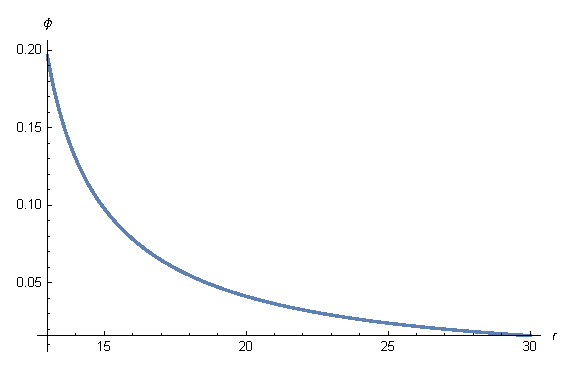
\includegraphics{images/geodesic.eps}
    \caption{$b=13$时测地线函数图像}\label{fig:geodesic} % label 用来在文中索引
\end{figure}

\section{赤道面光线追踪}
\subsection{Convention}
我们有常量$G$与$c$,设$G=c=1$,方程的长度单位为黑洞质量$\frac{GM}{c^2}=M$,史瓦西半径为$2M$。

\subsection{光子轨道近点(Closest Approach)}
测地线方程\eqref{eq:geodesic}有奇点,是光子轨道的近点 (Closest Approach),函数在近点不再连续,所以我们需要计算近点$r3$,
\begin{equation}
    b=\frac{r_3}{\sqrt{1-\frac{r_s}{r_3}}}\label{eq:r3}
\end{equation}
这是一个三次方程,需要根据光子的发射距离$r$决定方程的根,其中$r_s=\frac{2GM}{c^2}$为史瓦西半径。积分路径上第一个不连续的点就是轨道的近点。

\subsection{撞击参数与光子发射角}
光线是从光源传向镜头,被镜头捕捉后成像。但传统光线追踪是逆向追踪,光线从镜头出发,根据光线在镜头上的位置,以镜头上的不同角度散开,然后与远处的物体求交点。我们需要的起始参数是光线的相对于世界坐标的发射角度。

从测地线方程中可以看出撞击参数是唯一决定无质量粒子的运动轨迹的参数。我们要获得粒子运动轨迹与粒子发射角度、粒子发射距离的关系,需要重新推导这个关系式。
撞击参数$b$有如下定义,
\begin{equation}
    b=\frac{Lc}{E}
\end{equation}
其中$L$是角动量,$c$是真空光速,$E$是粒子的能量。$L$与$E$都是运动常量,光线出发时就可以确定。

\begin{equation}
    \begin{split}
        b&=\frac{Lc}{E}\\&=\frac{\vec{r}\times\vec{p}c}{E_{kinetic}+E_{Potential}}\\&=\frac{rp\sin\theta c}{hf+\left(\sqrt{1-\frac{r_{s}}{r}}-1\right)hf}\\&=\frac{rp\sin\theta c}{pc+\left(\sqrt{1-\frac{r_{s}}{r}}-1\right)pc}\\b&=\frac{r\sin\theta}{\sqrt{1-\frac{r_{s}}{r}}}\label{eq:impact_param}
    \end{split}
\end{equation}
其中$\vec{r}$是粒子的方向向量,$\vec{p}$是粒子的动量向量,光子没有静质量,所以我们得到光子的总能量是光子的动量$E_{kinetic}$与光子势能$E_{potential}$。这样我们就得到了发射距离$r$、发射角$\theta$与撞击参数$b$的关系。

\paragraph{圆周轨道}
从这个关系式\eqref{eq:impact_param}中,令光子的发射角度$\theta=\frac{\pi}{2}$可以得到光子的圆周轨道
\begin{equation*}
    \begin{split}
        \frac{b\sqrt{1-\frac{r_{s}}{r}}}{r}&=\sin\theta\\
        b&=\frac{3\sqrt{3}}{2}r_{s}\label{eq:circular_orbit}
    \end{split}
\end{equation*}
光子在史瓦西时空只有$r=3M$这一个不稳定圆周轨道。

\subsection{方位角积分图像}
设$r_0$为光子的出发距离,$r_1$为光子的最终距离,$r_3$为光子轨道近点,$\theta$为发射角度。$\Delta r$轴的前半部分(0-0.5)是光子发射点$r_0$到光子轨道近点$r_3$的线性比例距离,后半部分是近点$r_3$到设定的积分终点$r_1$的线性比例距离。函数横轴是分两段线性绘制的。横轴0.5处为轨道近点。纵轴$\Delta\phi$是积分原点$r_0$到$r$的积分,单位为弧度。
\begin{figure}[htbp]
    \centering
    \begin{subfigure}{.5\textwidth}
        \centering
        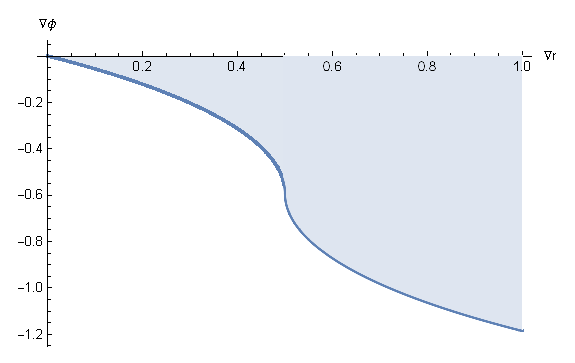
\includegraphics[width=.8\linewidth]{images/dphi_1.eps}
        \caption{$r_0=20M$, $r_1=20M$, $\theta=\frac{\pi}{3}$}\label{dphi_1} % label 用来在文中索引
    \end{subfigure}%
    \begin{subfigure}{.5\textwidth}
        \centering
        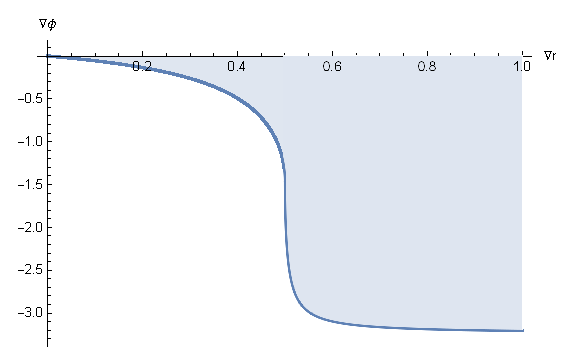
\includegraphics[width=.8\linewidth]{images/dphi_2.eps}
        \caption{$r_0=40M$, $r_1=400M$, $\theta=\frac{\pi}{10}$}\label{dphi_2} % label 用来在文中索引
    \end{subfigure}
\end{figure}

\subsection{轨道模拟}
假定光线在赤道面上运动,将三维运动简化为二维。中心天体半径为史瓦西半径$r_s=2M$。
可以得到光线在黑洞附近偏折的路径,下图近似为无限远处射出的光线经过黑洞再射向无限远处。可以看出光子发射角如果较小,会在距离黑洞较近的时候产生较大的偏转。

当撞击参数$b>\sqrt{27}$时\eqref{eq:circular_orbit},能得到类似\ref{fig:equatorial_plane_trace_1}的散射轨道。
\begin{figure}[htbp]
    \centering
    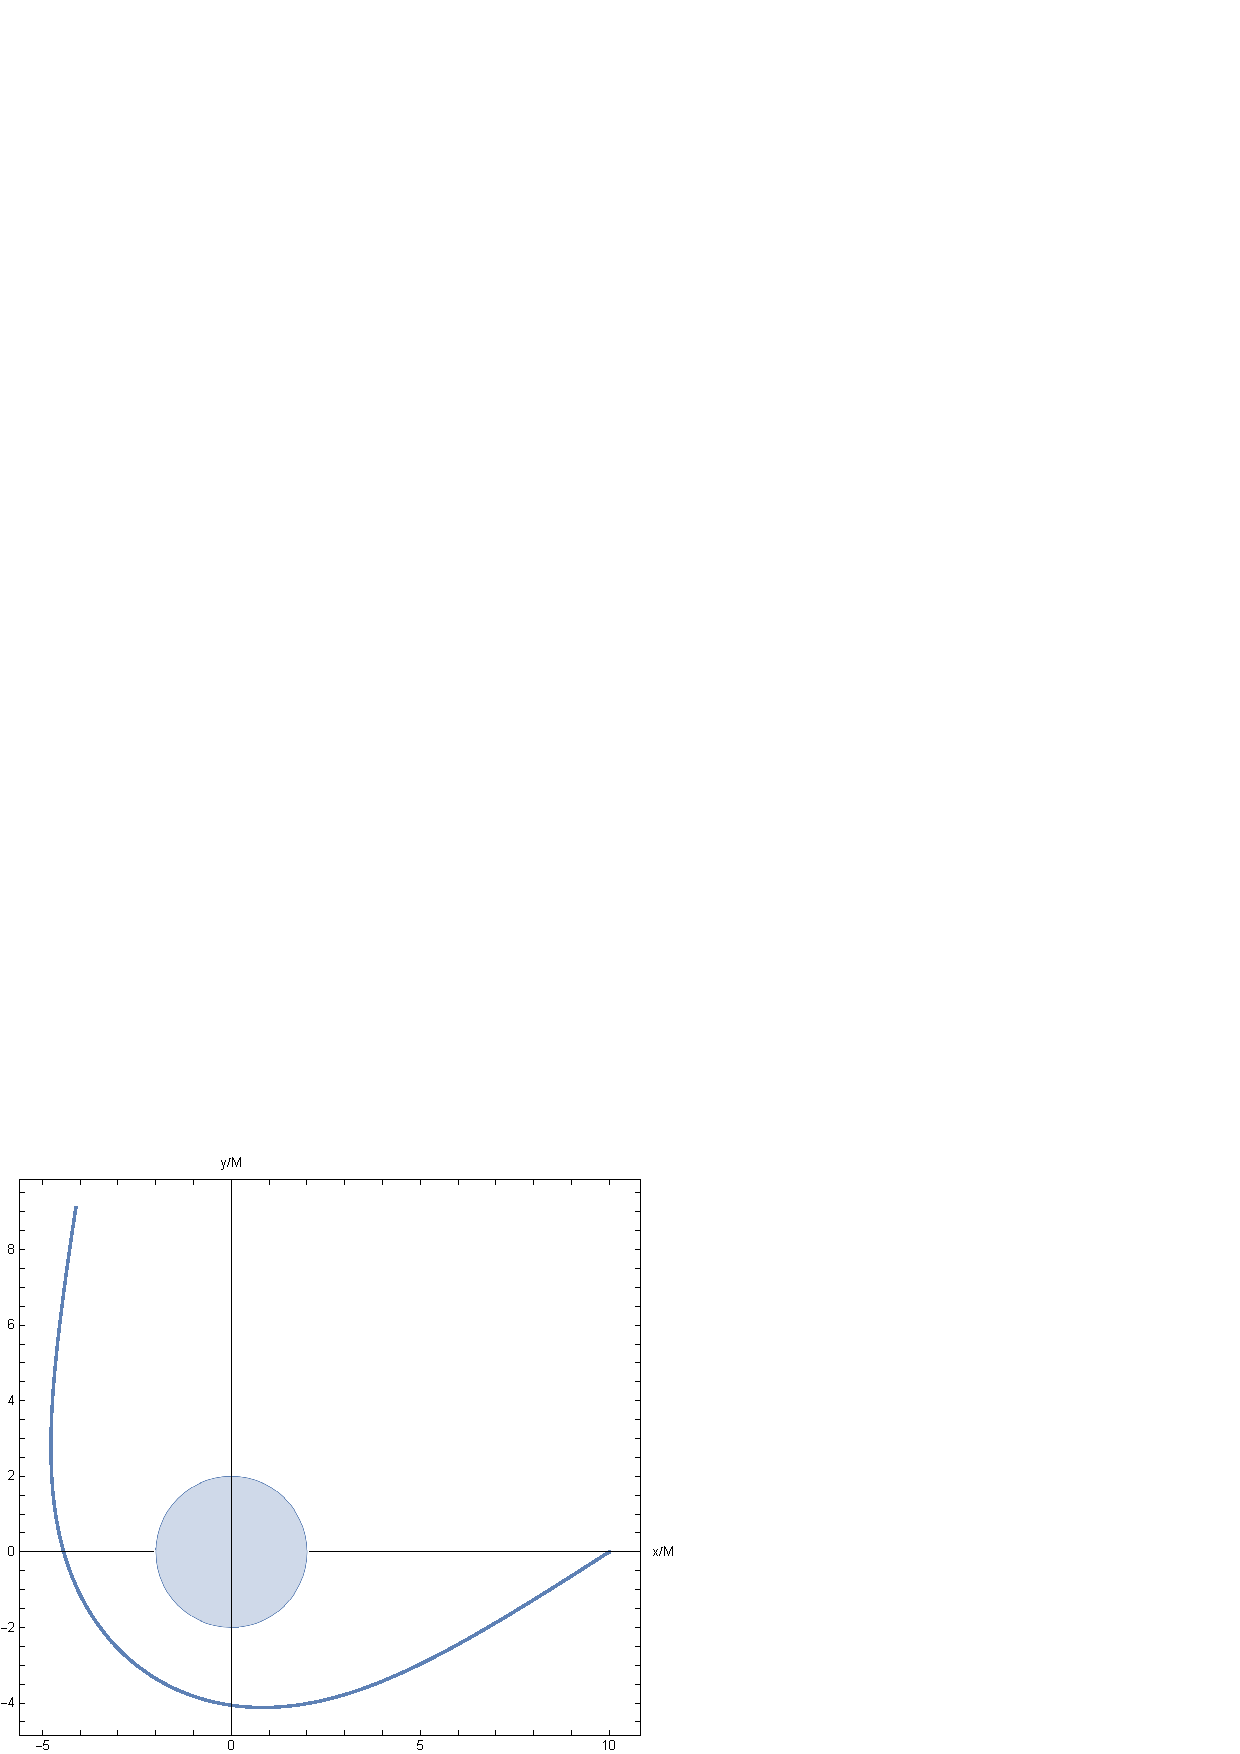
\includegraphics[scale=0.3]{images/equatorial_plane_trace_1.pdf}
    \caption{$r_0=50M$, $r_1=30M$, $\theta=\frac{\pi}{6}$}\label{fig:equatorial_plane_trace_1} % label 用来在文中索引
\end{figure}


当$b<\sqrt{27}$,会得到类似下图的坠入轨道。光线从相机出发,最终坠入黑洞.\begin{figure}[H]
    \centering
    \includegraphics[scale=0.3]{images/equatorial_plane_trace_2.pdf}
    \caption{$r_0=5M$, $b=5$}\label{fig:equatorial_plane_trace_2} % label 用来在文中索引
\end{figure}

当$b$非常接近$\sqrt{27}$时,光线会进入黑洞的光球区域$r=3M$,也就是史瓦西黑洞的唯一光子圆周轨道。光球汇集了来自各个方位的光子,它们会在这个区域盘旋。但这个轨道是不稳定的,最终光子会坠入黑洞,或者逃离黑洞。
\begin{figure}[htbp]
    \centering
    \begin{subfigure}{.5\textwidth}
        \centering
        \includegraphics[width=.9\linewidth]{images/photon_sphere_orbit_1.pdf}
        \caption{$r_0=10M$, $r_1=30M$, $b=\sqrt{27.002}$光子逃离}\label{dphi_1} % label 用来在文中索引
    \end{subfigure}%
    \begin{subfigure}{.5\textwidth}
        \centering
        \includegraphics[width=.9\linewidth]{images/photon_sphere_orbit_2.pdf}
        \caption{$r_0=10M$, $b=\sqrt{26.998}$光子被捕获}\label{dphi_2} % label 用来在文中索引
    \end{subfigure}
\end{figure}
以上情形适用于光子发射距离大于3M,小于3M的情形这里不再详述。

\paragraph{可能进入相机的光线}
下图描绘了一个在距离黑洞5M,斜$\ang{45}$角面向黑洞,拥有$\ang{90}$视场的相机所能获取的光线范围。相机可以获得平面内来自任意方向的光线,来自相机背后的光线会被压缩在一片很小的区域。
\begin{figure}[H]
    \centering
    \includegraphics[scale=0.5]{images/camera_view_orbit.pdf}
    \caption{$r=5M$, $FoV=\ang{90}$}\label{fig:camera_view_orbit} % label 用来在文中索引
\end{figure}